\documentclass[a4paper,11pt,dvipdfmx]{ujarticle}
% パッケージ
\usepackage{graphicx}
\usepackage{url}
% レイアウト指定を記述したファイルの読み込み
\input{layout}

% タイトルと氏名を変更せよ.
\title{日本におけるデジタル化の状況}
\author{G584572025 高浜 光来}

\begin{document}

\maketitle 

\section{デジタル競争力ランキング}

国際経営開発研究所(IMD)の調査\cite{imd}によると, 
日本のデジタル競争力のランキングは図\ref{zu.png}に示すように,
調査対象の64カ国中,総合で28位,技術分野で30位となっている.

\begin{figure}[htbp]
    \centering
    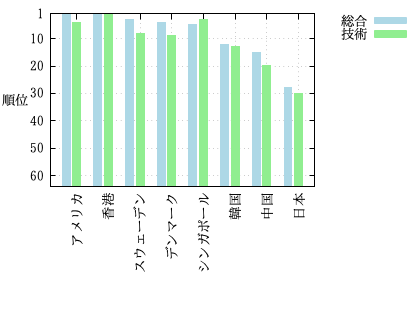
\includegraphics[width=0.7\linewidth]{zu.png}
    \caption{デジタル競争力ランキング(64カ国中)}\label{zu.png}
\end{figure}

\section{ブロードバンドの整理状況}

OECDによるブロードバンド回線の普及に関する調査\cite{oecd}
によると,表\ref{tbl:加入者数}に示すように,日本における100人
あたりのモバイルブロードバンドの加入者数は190.5で,
第1位になっている.
2位はエストニアで,3位米国と続く.

\begin{table}[htbp]
    \centering
    \caption{モバイルブロードバンドの加入者数(100人あたり)}
    \label{tbl:加入者数}

    \begin{tabular}{|c|l|r|}
        \hline
        順位 & 国名 & 加入者数 \\
        \hline
        1位 & 日本 & 190.5 \\
        \hline
        2位 & エストニア & 179.9 \\
        \hline
        3位 & 米国 & 169.0 \\
        \hline
        4位 & フィンランド & 157.0 \\
        \hline
        5位 & デンマーク & 141.7 \\
        \hline
        6位 & ラトビア & 141.6 \\
        \hline 
        7位 & イスラエル & 139.9 \\
        \hline
        8位 & オランダ & 133.7 \\
        \hline
        9位 & ポーランド & 131.3 \\
        \hline
        10位 & スウェーデン & 127.2 \\
        \hline
    \end{tabular}
\end{table}

\section{考察}

\begin{itemize}
    \item デジタル競争ランキングを見ると
    日本のデジタル競争力は他国に大きく劣っている.
    \item ブロードバンドの整理状況を見ると,
    日本のモバイルブロードバンドの加入者数は
    2位と大差をつけて1位になっている.
\end{itemize}

\bibliographystyle{junsrt}
\bibliography{exercise.bib}

\end{document}